%%%%%%%%%%%%%%%%%%%%%%%%%%%%%%%%%%%%%%%%%%%%%%%%%%%%%%%%%%%%%%%%%%%%%%
% LaTeX Template: Two Column Colour Article
%
% Source: http://www.howtotex.com/
% Feel free to distribute this template, but please keep the
% referal to howtotex.com.
% Date: Feb 2011
%%%%%%%%%%%%%%%%%%%%%%%%%%%%%%%%%%%%%%%%%%%%%%%%%%%%%%%%%%%%%%%%%%%%%%
% adaptions made by wolfgang stoettner mail@stoettner.net
%%%%%%%%%%%%%%%%%%%%%%%%%%%%%%%%%%%%%%%%%%%%%%%%%%%%%%%%%%%%%%%%%%%%%%

%%% Preamble
\documentclass[	DIV=calc,%
							paper=a4,%
							fontsize=10pt,%
							twocolumn]{scrartcl} % KOMA-article class
\usepackage[french]{babel}	% English language/hyphenation
\usepackage[protrusion=true,expansion=true]{microtype}	% Better typography
\usepackage{amsmath,amsfonts,amsthm} % Math packages
\usepackage{pythontex} % Math packages
\usepackage[pdftex]{graphicx} % Enable pdflatex
\usepackage{wrapfig} % enable figure wrapping
\usepackage[svgnames]{xcolor} % Enabling colors by their 'svgnames'
\usepackage[hang, small,labelfont=bf,up,textfont=it,up]{caption} % Custom captions under/above floats
\usepackage{epstopdf} % Converts .eps to .pdf
\usepackage{subfig}	% Subfigures
\usepackage{booktabs} % Nicer tables
\usepackage{fix-cm}	% Custom fontsizes
\usepackage{booktabs} % prof. looking tables (www.en.wikibooks.org/wiki/LaTeX/Tables#Professional_tables)
\usepackage{float}
\usepackage{tgtermes}
\usepackage[T1]{fontenc}
\usepackage[utf8]{inputenc}
\usepackage{pdfpages}
\usepackage[smartEllipses]{markdown}
\usepackage[top=1.5cm, bottom=1cm, left=1cm, right=1cm, showframe=false]{geometry}

%%% Custom sectioning (sectsty package)
\usepackage{sectsty} % Custom sectioning (see below)
\allsectionsfont{%		% Change font of al section commands
	\usefont{OT1}{phv}{b}{n}%	% bch-b-n: CharterBT-Bold font
	}

\sectionfont{%		% Change font of \section command
	\usefont{OT1}{phv}{b}{n}%	% bch-b-n: CharterBT-Bold font
	}
%%% Headers and footers
\usepackage{fancyhdr} % Needed to define custom headers/footers
	\pagestyle{fancy} % Enabling the custom headers/footers
\usepackage{lastpage}	

% Header (empty)
\lhead{}
\chead{}
\rhead{}
% Footer (you may change this to your own needs)
\lfoot{\footnotesize \texttt{formulaire mécatronique 2} \textbullet \vspace{5pt} Antonin Kenzi}
\cfoot{}
\rfoot{\footnotesize page \thepage\ of \pageref{LastPage}}	% "Page 1 of 2"
\renewcommand{\headrulewidth}{0.0pt}
\renewcommand{\footrulewidth}{0.4pt}
\newcommand{\hformbar}[1]{\bigskip \hrule \vspace{1pt} \hrule \vspace{5pt}} % creates a horizontal bar to separate formulae better; space adaptions can be made centrally here


%%% Creating an initial of the very first character of the content
\usepackage{lettrine}
\newcommand{\initial}[1]{%
     \lettrine[lines=3,lhang=0.3,nindent=0em]{
     				\color{DarkGoldenrod}
     				{\textsf{#1}}}{}}

%%% Title, author and date metadata
\usepackage{titling} % For custom titles

\newcommand{\HorRule}{\color{DarkGoldenrod}%	% Creating a horizontal rule
									  	\rule{\linewidth}{1pt}%
										}
\pretitle{\vspace{-83pt} \begin{flushleft} \HorRule 
				\fontsize{15}{15} \usefont{OT1}{phv}{b}{n} \color{DarkRed} \selectfont 
				}
\title{Formulaire mécatronique 2} % Title of your article goes here
\posttitle{\par\end{flushleft}}
\preauthor{\vspace{-20pt} \begin{flushleft}\large \usefont{OT1}{phv}{b}{sl} \color{DarkRed}}
\author{Kenzi Antonin}	% Author name goes here
\postauthor{\vspace{-20pt} \footnotesize \usefont{OT1}{phv}{m}{sl} \color{Black}  \par\end{flushleft}\HorRule}
\date{\vspace{-30pt} \today} % No date
\newcounter{mycounter}
%%% wws: create a non-indented formula name
\newcommand{\formdesc}[1]{\large\textbf{#1} \addtocounter{mycounter}{1} \hfill \themycounter \\ \vspace{-3mm} \hrule \vspace{2mm}}

\newcommand{\formtitle}[1]{\large\underline{#1}}
\setlength\parindent{0pt}

%%% Begin document -----------------------------------------------------------------
\begin{document}
\maketitle
\thispagestyle{fancy} 	% Enabling the custom headers/footers for the first page 
% The first character should be within \initial{}

\formdesc{Moteur à courant continu}
\begin{enumerate}
    \item Stator : fixe
    \item Rotor : mobile
    \item Collecteur : élément d'usure 
\end{enumerate}

\formtitle{Production de couple :}
\begin{itemize}
    \item spire parcourue par un courant $i_a(t)$
    \item Champ d'induction B 
\end{itemize}
Par Laplace :

{\hfill $\vec{F} = (\vec{i_a}(t) \wedge  \vec{B})\cdot l$\hfill}

cette force produit un couple faisant tourner le moteur : 

{\hfill $T_{em}(t) = k_T \cdot i_a(z)$\hfill}

cela induit une tension :

{\hfill $u_i(t) = \cfrac{d \Phi(t)}{dt}=k_u \cdot \omega(t)$\hfill}

\hformbar

\formdesc{Équations du moteur Dc et de la charge}

{ \vspace{-3mm}
    \begin{figure}[H]
        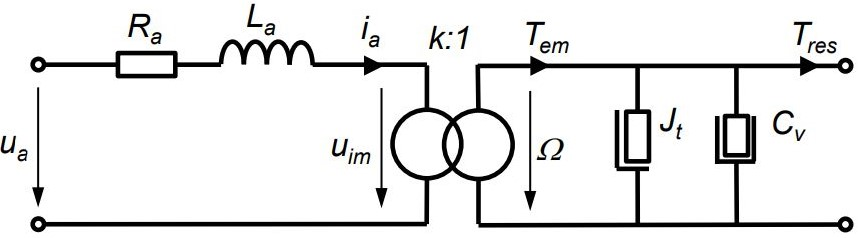
\includegraphics[width=0.45\textwidth]{img/equation_mot.JPG}
    \end{figure}
}
\formtitle{Équation de tension : }

{\hfill $u_a(t) = R_a \cdot i_a + L_a \cfrac{di_a(t)}{dt}+u_{im}(t)$\hfill}

{\hfill $I_a(s) = [U_a(s).U_{im}(s)] \cdot \cfrac{ \cfrac{1}{R_a}}{1+s\cfrac{L_a}{R_a}}  $\hfill}


\formtitle{Équation de mouvement :} 

{\hfill $Jt \cfrac{d\Omega(t)}{dt} = T_{em}(t) - C_v \Omega(t) - Tres(t) $\hfill}

{\hfill $\Omega(s) = [T_{em}(s).T_{res}(s)] \cdot \cfrac{ \cfrac{1}{C_v}}{1+s\cfrac{J_t}{C_v}}  $\hfill}

\formtitle{Équation de couplage : }

{\hfill $k_T = \cfrac{T_{em}(t)}{i_a(t)} = \cfrac{u_{im}(t)}{\Omega(t) }= k_u$\hfill}

\formtitle{Hypothèses :}
\begin{enumerate}
    \item Linéarité : pas de saturation du fer, résistance Cst
    \item Frottements négligeables, généralement < 5\% du couple nominal
    \item arbre rigide en torsion : ce n’est pas toujours le cas
\end{enumerate}

\formdesc{Calcul des fonctions de transfert}

on introduit :
\begin{itemize}
    \item $\tau_e = \cfrac{L_a}{R_a}$
    \item $\tau_m = \cfrac{J_t\cdot R_a}{k_T\cdot k_E}$
\end{itemize}

Les fonctions de transfert du moteur DC et de la charge, sans frottements visqueux, deviennent :


{\hfill $G_{u\omega} = \cfrac{\Omega(s)}{U_a(s)} = \cfrac{1}{k_E}\cdot\cfrac{1}{1 + s \cdot \tau_m + s^2 \cdot \tau_m \cdot \tau_e} $\hfill}

\vspace{3mm}
{\hfill $G_{ui} = \cfrac{I_a(s)}{U_a(s)} = \cfrac{J_t}{k_E\cdot k_T}\cdot\cfrac{1}{1 + s \cdot \tau_m + s^2 \cdot \tau_m \cdot \tau_e} $\hfill}

\vspace{3mm}

\formtitle{Cas particulier : $\tau_m \leqslant 4 \cdot\tau_e$}

Dénominateur défini par 2 pôles réels :

\vspace{3mm}
{\hfill $s_{1,2} = \cfrac{-\tau_m \pm \sqrt{\tau_m^2 - 4 \cdot \tau_m \cdot \tau_e}}{2 \cdot \tau_m \cdot \tau_e} $\hfill}

\vspace{3mm}
ce qui décompose le système tel que : 

{\hfill $ \cfrac{1}{(1+s\cdot \tau_{max})(1+s\cdot \tau_{min})}$\hfill}
avec : {\hfill $\tau_{max,min} = -\cfrac{1}{s_{1,2}}$\hfill}

\vspace{3mm}
\formtitle{Cas particulier : $\tau_m \ggg \tau_e $}
{\hfill $ \cfrac{1}{(1+s\cdot \tau_{m})(1+s\cdot \tau_{e})}$\hfill}


\formtitle{Fonction page 1.22 :}

\hformbar


\formdesc{Alimentations des moteurs DC}

\formtitle{Méthodes :}

\begin{enumerate}
    \item Analogique : Grande perte à basse vitesse. 
    \item Alimentation à découpage : pertes variateur constant
\end{enumerate}

\formtitle{Pont en « H » :}

\begin{figure}[H]
    \begin{center}      
        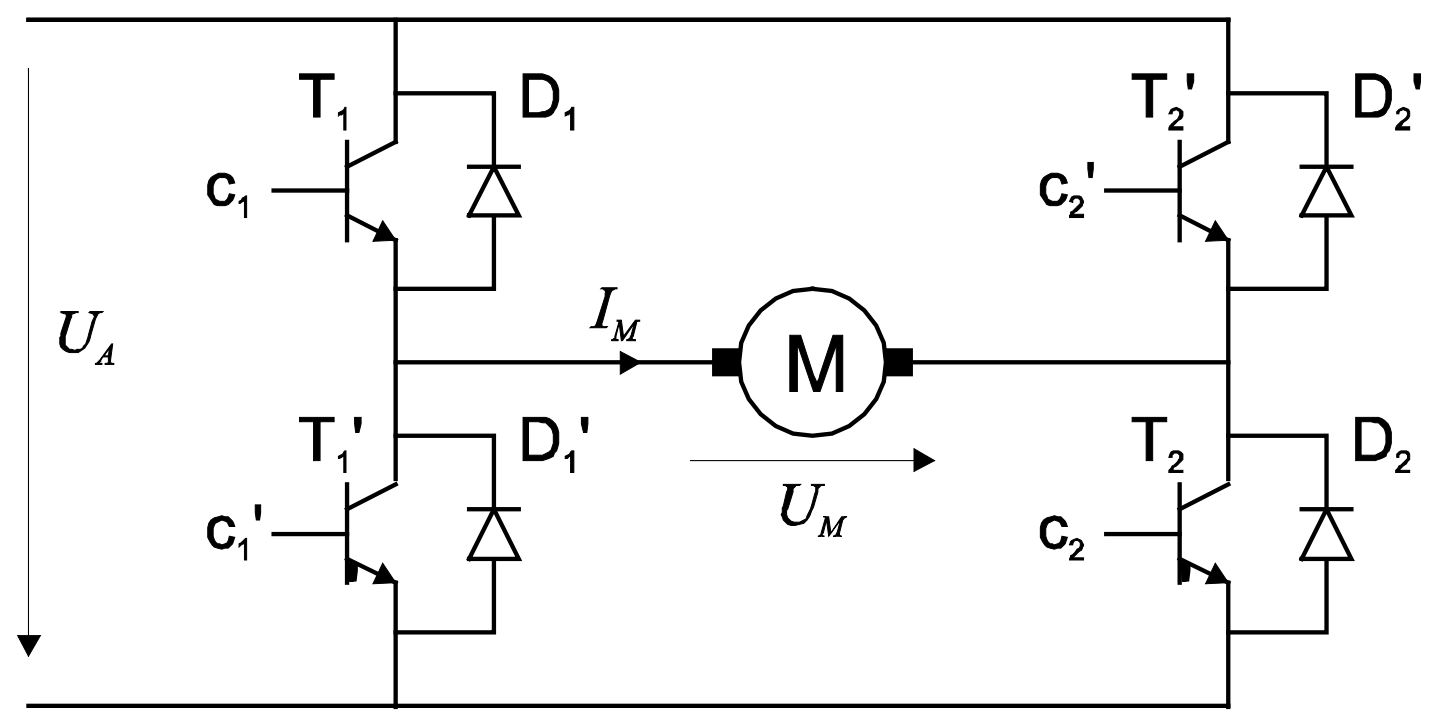
\includegraphics[width = 0.3\textwidth]{img/Pont_H.JPG}
    \end{center}
\end{figure}
\formtitle{Gestion par pulse width modulation}

\begin{enumerate}
    \item \formtitle{Par régime stationnaire : }

{\hfill $ \bar{U_{M}} = U_A * \biggl(2 \cdot \cfrac{t_e}{T_P} -1 \biggr)$\hfill}

\item \formtitle{Par «sous-oscillation» : }

\item \formtitle{Par fonction de transfert : }

    \begin{figure}[H]
        \begin{center}      
            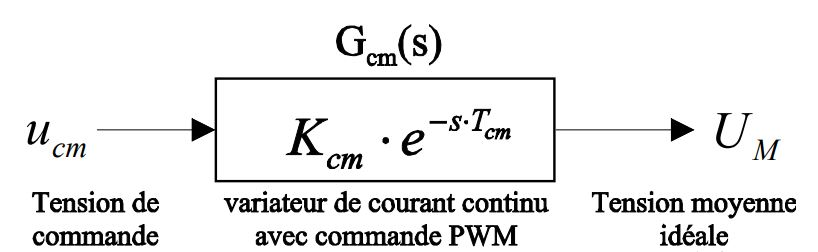
\includegraphics[width = 0.4\textwidth]{img/PWM_FT.JPG}
        \end{center}
    \end{figure}

    {\hfill $ K_{cm} = \cfrac{U_A}{\hat{u_{cm}}}$\hfill}

\end{enumerate}

\formtitle{Approximation du retard pur : }
\begin{itemize}
    \item Si analogique 
        \begin{itemize}
            \item $u_h$ triangulaire : $T_{cm} = \cfrac{T_p}{3} $
            \item $u_h$ dent de scie : $T_{cm} = \cfrac{T_p}{2} $
        \end{itemize}
    \item Si Numérique : $T_{cm} = T_p $
\end{itemize}



\begin{table}
    \begin{tabular}{c | c}
        1er ordre : & Padé : \\
        {\hfill $ e^{-s\cdot T_{cm}} \backsimeq \cfrac{1}{1 + s\cdot T_{cm}} $\hfill} & {\hfill $ e^{-s\cdot T_{cm}} \backsimeq \cfrac{1 - s \cdot \cfrac{T_{cm}}{2}}{1 + s \cdot \cfrac{T_{cm}}{2}} $\hfill}
    \end{tabular}
\end{table}


\hformbar


\formdesc{Rappel sur le moment d’inertie}

\begin{figure}[H]
    \begin{center}      
        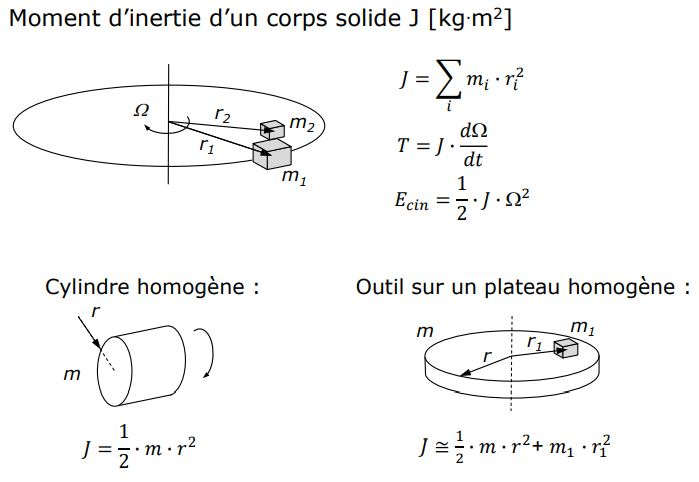
\includegraphics[width = 0.49\textwidth]{img/Rappel_inertie1.JPG}
    \end{center}
\end{figure}

Courroie ou crémaillère : $J_{eq} = m \cdot r^2$

{\centering 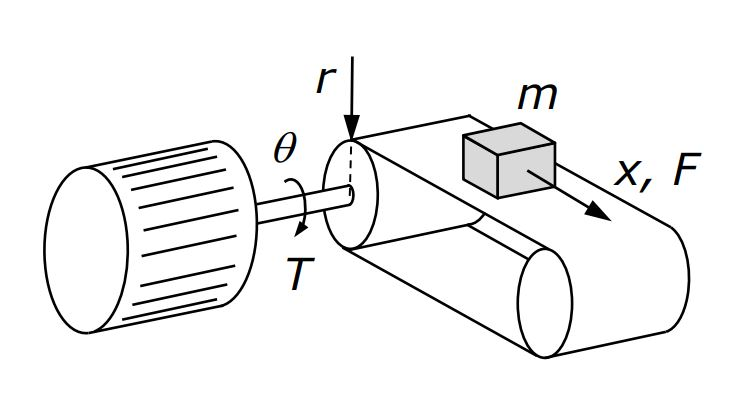
\includegraphics[width = 0.3\textwidth]{img/Cremaillere.JPG}}

\vspace{1cm}

Vis-à-billes : $J_{eq} = m \cdot \biggl(\cfrac{p}{2\pi}\biggr)^2$

{\centering 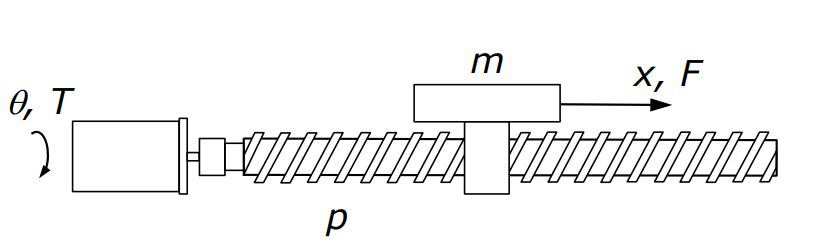
\includegraphics[width = 0.3\textwidth]{img/vis.JPG}}

Réducteurs : $J_{eq} = J_{ch}\cdot \cfrac{1}{i^2} $ \quad avec $ i = \cfrac{\Omega_m}{\Omega_e}$ 

{\centering 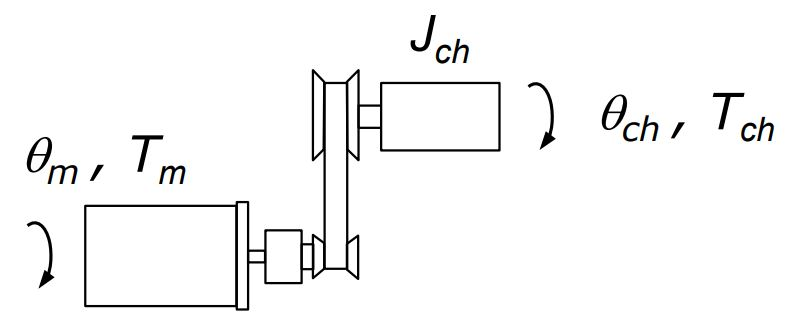
\includegraphics[width = 0.3\textwidth]{img/Reducteur.JPG}}

\hformbar

\formdesc{Réglage du courant / couple}
\begin{figure}[H]
    \begin{center}
        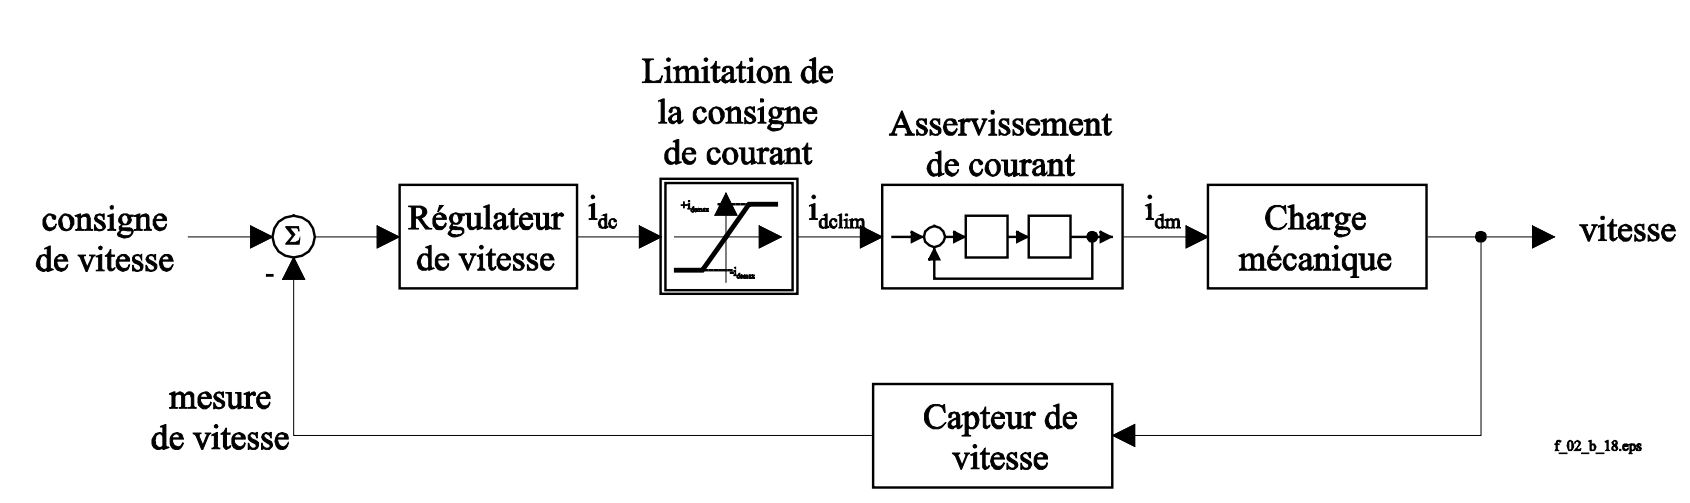
\includegraphics[width = 0.49\textwidth]{img/Regulation_courrant.JPG}

        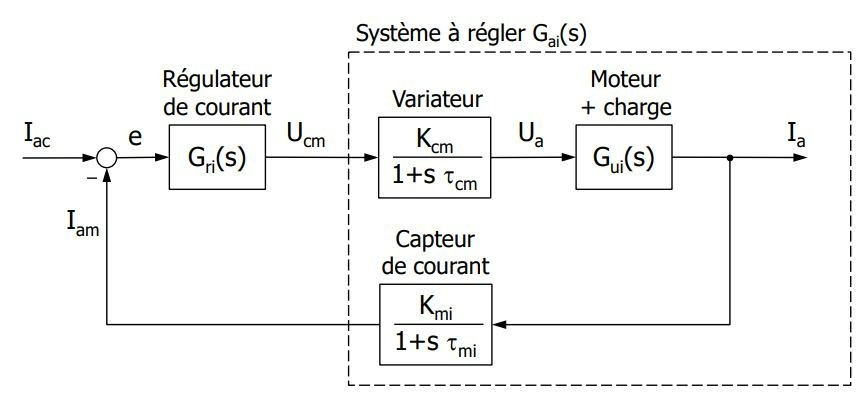
\includegraphics[width = 0.4\textwidth]{img/Regulation_courrant_Gai.JPG}

    \end{center}
\end{figure}

{\footnotesize $G_{ai}(s) = K_{ai} \cdot \cfrac{s}{1+s \cdot \tau_m + s^2 \cdot \tau_e \cdot \tau_m} \cdot \cfrac{1}{1+s \cdot \tau_{cm}}\cdot \cfrac{1}{1+s \cdot \tau_{mi}} $}

\vspace{3mm}

{\footnotesize$K_{ai} = \cfrac{K_{cm} \cdot K_{mi} \cdot J_t}{k_t \cdot k_E}$}

\hformbar

\formdesc{Régulateur PI}

\begin{itemize}
    \item composante I    
        \begin{itemize}
            \item pour compenser le comportement dérivateur à basses fréquences
            \item pour compenser les couples perturbateur à moyennes fréquences
        \end{itemize}
    \item composante P  
    \begin{itemize}
        \item pour annuler la composante I en hautes fréquences donc, pour ne pas trop dégrader la bande passante
    \end{itemize}
\end{itemize}

\formtitle{fonction de transfert en boucle ouverte : }

\vspace{3mm}

{ $G_{reg,{PI}}(s) =  K_{PI} \cdot \cfrac{1+s\cdot\tau_{ii}}{s\cdot\tau_{ii}} \cdot G_{ai}(s) $}

\vspace{3mm}

\formtitle{Ajustage traditionnel (compensation du pôle dominant)}

\vspace{3mm}
$\tau_{ii} = \tau_{dominant}$
\vspace{3mm}

\underline{Problème :}
\begin{itemize}
    \item  erreur statique importante ($~27\%$)
\end{itemize}

\formtitle{Ajustage sur les petites constantes de temps}

\vspace{3mm}
$\tau_{ii} = N \cdot \sum\tau_{pct} = N \cdot (\tau_{cm}+ \tau_{mi})$ ,avec N $\leq$ 10 [5...30]

\underline{Avantages :}
\begin{itemize}
    \item Système en boucle fermée avec $K_{pi} = +13 dB$
    \item Erreur statique quasi nulle
    \item Bande passante quasi inchangée
\end{itemize}


\formdesc{régulation imbriquée position – courant}
\begin{figure}[H]
    \begin{center}
        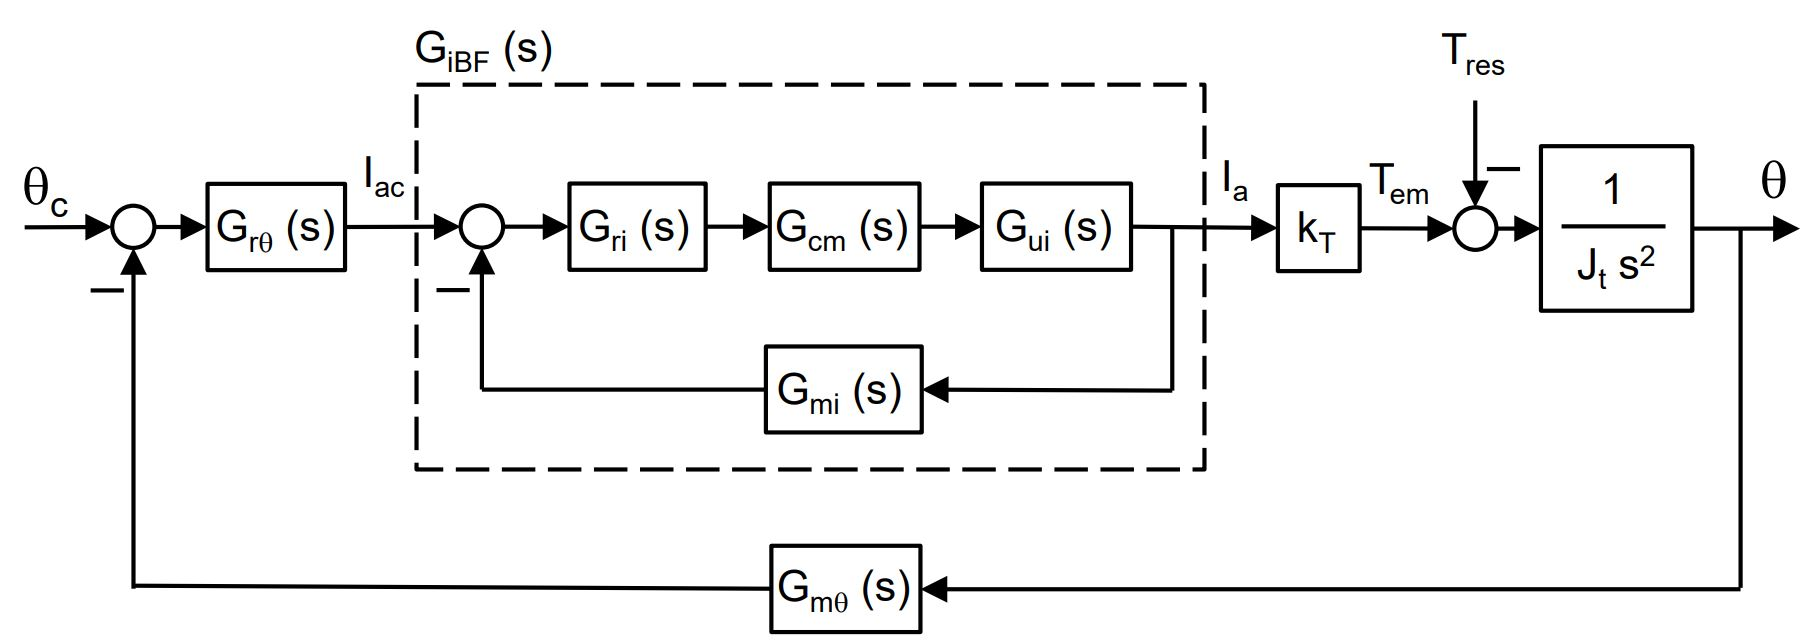
\includegraphics[width = 0.49\textwidth]{img/Regulation_courrant_pos.JPG}
    \end{center}
\end{figure}

\formtitle{Capteur de position}
\underline{Fonction de transfert  (approx.) :}

\vspace{3mm}
$G_{m\theta}(s) = \cfrac{K_{m\theta}}{1+s\cdot\tau_{m\theta}} $

$X_{commande} \cdot N_1 = X_{mesure} \cdot N_2$

$K_{m\theta} = N_2/N_1$

\underline{Unité de la consigne de courant}

Consigne exprimée en : 
\begin{itemize}
    \item Courant : $U_{ci} = I_c \cdot K'_{mi}$ avec $K'_{mi} \approxeq K_{mi}$
    \item Couple  : $U_{ci} = T_c \cdot K'_{mi}/k'_T$ avec $k'_T \approxeq k _T$
\end{itemize}


\underline{Boucle fermée de courant}

on peut utiliser la fonction de transfert en boucle fermée obtenue 
précédemment (calcul « exact »), ou on peut en faire une approximation du 1er ordre, dont la fonction de 
transfert es :

$G_{iBF}(s) = \cfrac{1}{1+s\cdot\tau_{iBF}} $

$G_{iBF}(0) \approxeq 1$

 $\tau_{iBF} = 1/ \omega_{m\varphi 45^\circ}$ 

\underline{Système à régler}

$G_{a\theta}(s) = \cfrac{\theta(s)}{I_{ac}(s)} = \underbrace{\cfrac{1}{1+s\cdot\tau_{iBF}}}_{G_{iBF}(s)}\cdot k_T \cdot \underbrace{\cfrac{1}{J_t}\cfrac{1}{s^2}}_{Charge} \cdot \underbrace{\cfrac{K_{m\theta}}{1+s\cdot\tau_{m\theta}}}_{Capt-pos} $ 
$G_{a\theta}(s) = \underbrace{\cfrac{K_{m\theta} \cdot k_T}{J_t}}_{K_{a\theta} }\cdot \cfrac{1}{1+s\cdot\tau_{iBF}} \cdot \cfrac{1}{1+s\cdot\tau_{m\theta}}$

\underline{Régulateur}

PD = $G_{r\theta} = K_{p\theta} \cdot (1+s\cdot\tau_{d\theta})$

\underline{Ajustage}

$\tau_{ref} = \sum\tau_i \text{ ou } 1/\omega_{ref} $ à -225°

$\tau_{d\theta} = N \cdot \tau_{ref}$

Puis ajuster $K_{p\theta}$ 0 dB pour $\omega$
correspondant à la marge de phase souhaitée.

\underline{limiteur de courant}

Il nécéssaire d'ajouter un limiteur de courant sur la consigne ce qui rend le système non-linéaire.


\underline{Réaction aux couples perturbateurs}

\resizebox{.5\textwidth}{!}
{
$G_{v\theta}(s) = \cfrac{\cfrac{1}{Jt \cdot s^2}}{1+\cfrac{1}{Jt \cdot s^2}\cdot \cfrac{K_{m\theta}}{1+s\cdot\tau_{m\theta}} \cdot K_{p\theta} \cdot (1+s\cdot\tau_{d\theta}) \cdot G_{iBF\cdot k_T}}$
}
\newpage


\formdesc{Rigidité statique d’asservissement}

$K = \lim\limits_{t \rightarrow \infty} \biggl[\cfrac{|T_{res}(t)|}{|e_\theta(t)|}\biggr] = \lim\limits_{s \rightarrow 0} \biggl[\cfrac{1}{|G_{\theta}(s)|}\biggr]$

en Statique 
$T_{em} = T_{res}$

$K = \lim\limits_{s \rightarrow 0}[G_{r\theta(s)}\cdot G_{iBF}\cdot k_T]$

si regulateur PD : 

$K = \lim\limits_{s \rightarrow 0}\biggl[K_{p\theta} \cdot (1+s\cdot\tau_{d\theta}) \cdot \cfrac{1}{1+s\cdot\tau_{iBF}} \cdot k_T\biggr] = K_{p\theta \cdot k_T}$

\underline{Dilemme du choix du coefficient N}

Bonne marge de phase : N grand

peu d'erreur statique : N petit \\

solution : ajouter un filtre de consigne.

$G_f\theta = \cfrac{1}{1+s\cdot\tau_{fc\theta}}$

ne détériore pas la réaction aux couples perturbateurs

Evite d'exciter les hautes fréquences par la consigne mais limite la rapidité de réaction aux sauts de consignes

\underline{Effet d’une composante I}

\begin{itemize}
    \item annulerait l’erreur statique
    \item convient avec rigidité statique d'asservissement $ K = \infty $
    \item provoque un bref écart de position lorsque le couple perturbateur disparait (overshoots)
    \item à éviter lorsqu'il s'agit de garantir un suivi de consigne à forte dynamique
\end{itemize}


\formdesc{Commande a priori}

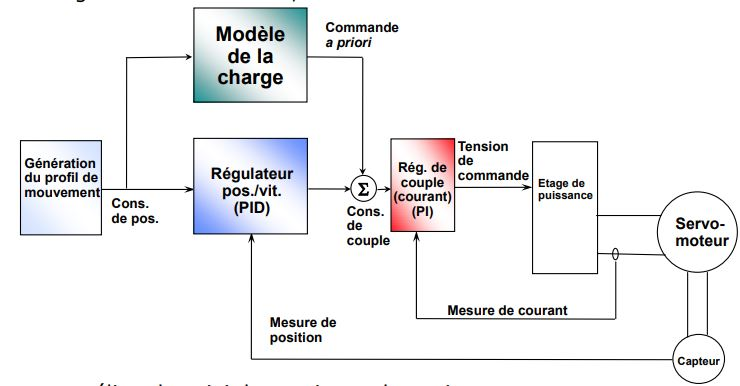
\includegraphics[width=0.49\textwidth]{img/com_apriorie.JPG}

Connaisance parfaite de la réaction du système 

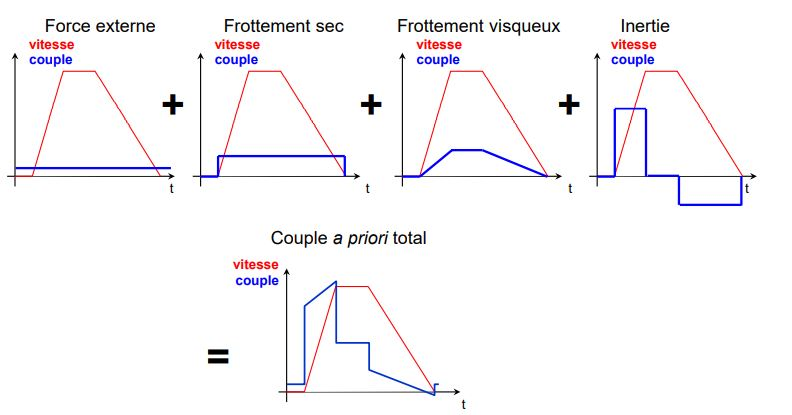
\includegraphics[width=0.49\textwidth]{img/com_apriorie_2.JPG}

\newpage

\formdesc{Standard de facto ( >95\% des cas)}

Régulateur ajustés séparement :

$\rightarrow $ régulateur de courant, en fonction du moteur

$\rightarrow $ régulateur de vitesse, en fonction de la charge mécanique

$\rightarrow $ régulateur de position, pour assurer la rigidité parfois exploitant un autre capteur (en aval du réducteur)

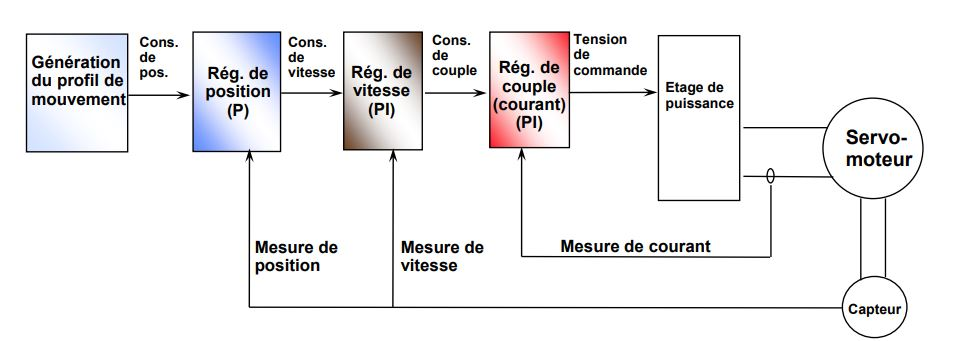
\includegraphics[width=0.49\textwidth]{img/stad_facto.JPG}


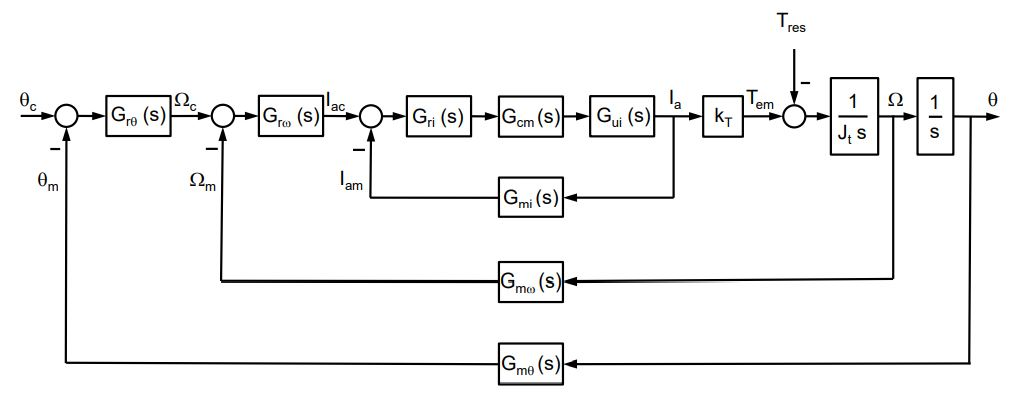
\includegraphics[width=0.49\textwidth]{img/stad_facto_2.JPG}

\formdesc{Arbre élastique }

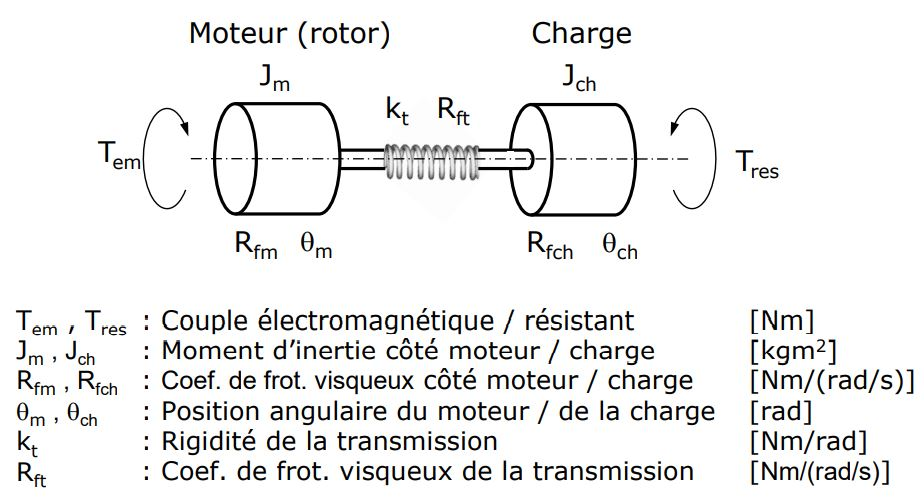
\includegraphics[width=0.49\textwidth]{img/arbre_elastique.JPG}

$\cfrac{\theta_m(s)}{T_{em}(s)} = \cfrac{s^2\:J_{ch} + s(R_{ft} + R_{fch}) + k_t}{a_4\: s^4 + a_3\: s^3 + a_2 \:s^2 + a_1 \:s}$\\
{\centering
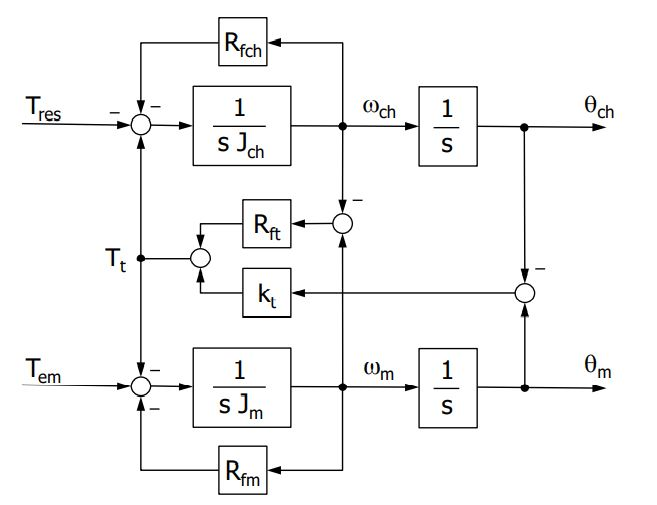
\includegraphics[width=0.3\textwidth]{img/arbre_elastique_2.JPG}
}
avec :\\
{\normalsize
$
    \begin{aligned}
        a_4 &= J_m \cdot J_{ch}\\
        a_3 &= J_m \cdot  (R_{ft} + R_{fch}) + J_{ch} \cdot (R_{ft} + R_{fm})\\
        a_2 &= (J_m + J_{ch})\cdot k_t + (R_{fch} + R_{fm}) \cdot R_{ft} + R_{fch} \cdot R_{fm}\\
        a_1 &= J_m \cdot j_{ch}\\
    \end{aligned}
$
}
avec simplification : 
{\normalsize
$
    \begin{aligned}
        a_4 &= J_m \cdot J_{ch}\\
        a_3 &=( J_m + J_{ch}) \cdot R_{fe}\\
        a_2 &= (J_m + J_{ch})\cdot k_t\\
        a_1 &= 0\\
    \end{aligned}
$
}

$R_{fe} = \cfrac{J_m \: R_{fch} + J_{ch}\:R_{fm}}{J_m + J_{ch}} + R_{ft}$


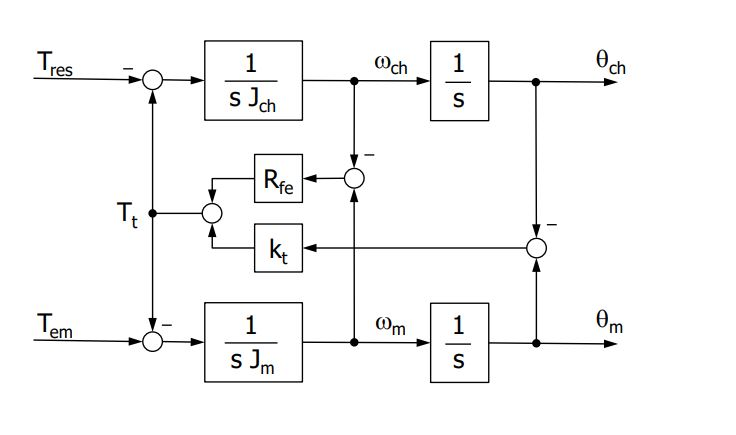
\includegraphics[width=0.49\textwidth]{img/arbre_elastique_3.JPG}

{\normalsize
$\cfrac{\theta_m(s)}{T_{em}(s)} = \cfrac{s^2\:J_{ch} + s\:R_{fe} + k_t}{J_mJ_{ch}\: s^4 + R_{fe}(J_m+J_{ch})\: s^3 + k_t(J_m+J_{ch}) \:s^2 }$\\


$\cfrac{\theta_{ch}(s)}{T_{em}(s)} = \cfrac{s\:R_{fe} + k_t}{J_mJ_{ch}\: s^4 + R_{fe}(J_m+J_{ch})\: s^3 + k_t(J_m+J_{ch}) \:s^2 }$\\


$\cfrac{\theta_{ch}(s)}{\theta_m(s)} = \cfrac{s\:R_{fe} + k_t}{s^2\: J_ch + s\:R_{fe} + k_t}$\\
}

\formtitle{Réponse harmonique}

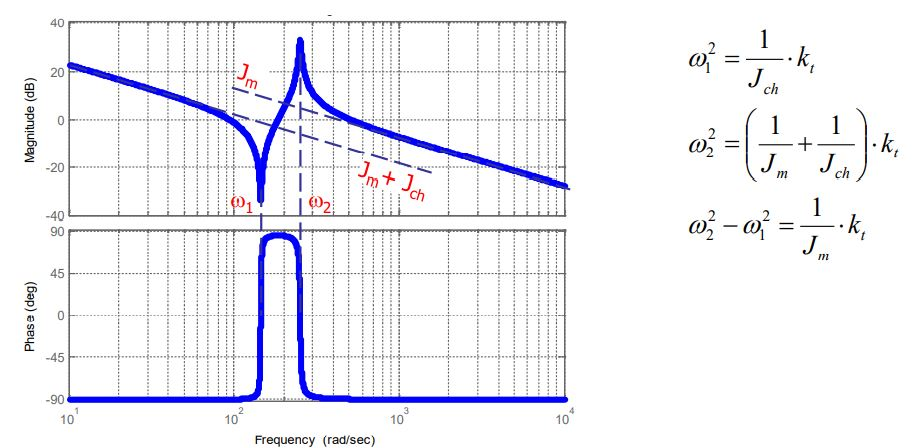
\includegraphics[width=0.49\textwidth]{img/arbre_elastique_rep.JPG}


\formtitle{Effet de l’arbre élastique en régulation de courant}

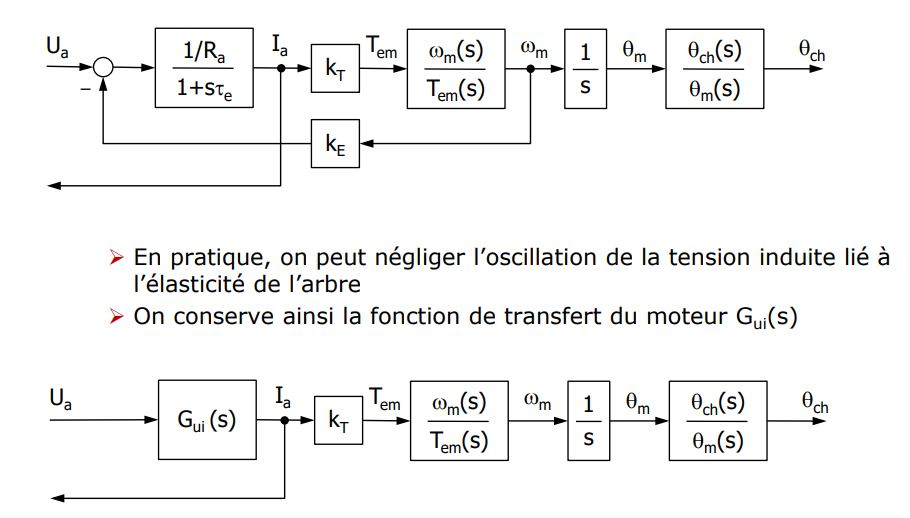
\includegraphics[width=0.49\textwidth]{img/arbre_elastique_bloc.JPG}


\formtitle{Effet de l’arbre élastique en régulation de vitesse}

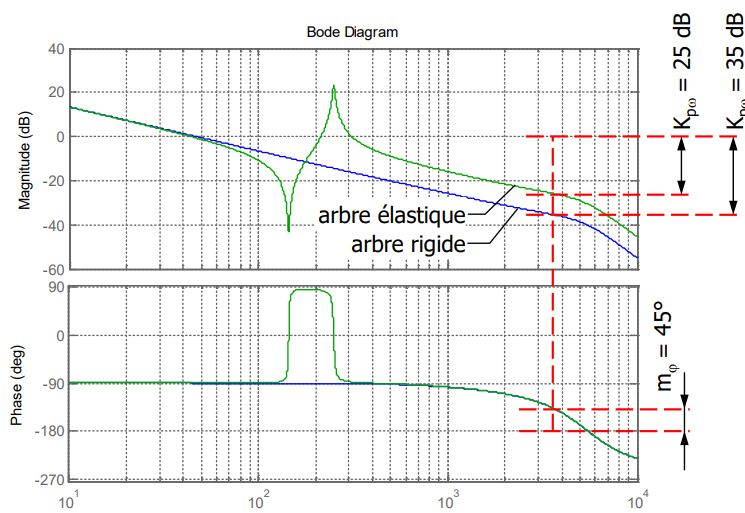
\includegraphics[width=0.49\textwidth]{img/arbre_elastique_vit.JPG}


\formtitle{Effet de l’arbre élastique en régulation de position}
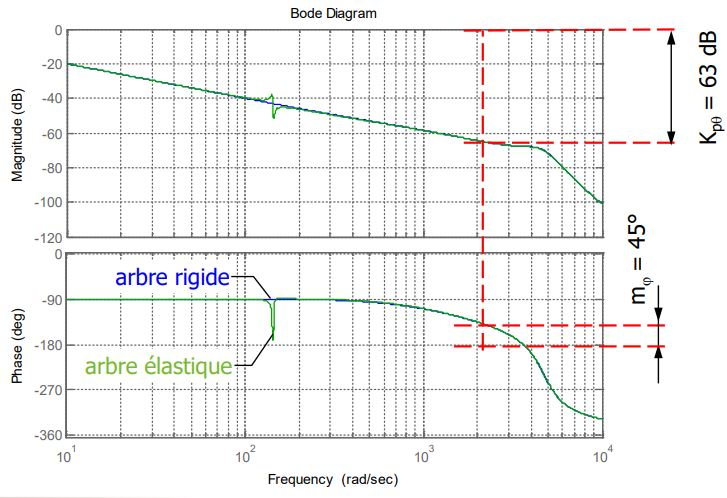
\includegraphics[width=0.49\textwidth]{img/arbre_elastique_pos.JPG}


\newpage

\formdesc{Rappel : }

\formtitle{Équation de tension : }

{\hfill $u_a(t) = R_a \cdot i_a + L_a \cfrac{di_a(t)}{dt}+u_{im}(t)$\hfill}

{\hfill $I_a(s) = [U_a(s).U_{im}(s)] \cdot \cfrac{ \cfrac{1}{R_a}}{1+s\cfrac{L_a}{R_a}}  $\hfill}


\formtitle{Équation de mouvement :} 

\vspace{3mm}

{\hfill $Jt \cfrac{d\Omega(t)}{dt} = T_{em}(t) - C_v \Omega(t) - T_{res}(t) $\hfill}

{\hfill $\Omega(s) = [T_{em}(s).T_{res}(s)] \cdot \cfrac{ \cfrac{1}{C_v}}{1+s\cfrac{J_t}{C_v}}  $\hfill}

\formtitle{Équation de couplage : }

{\hfill $k_T = \cfrac{T_{em}(t)}{i_a(t)} = \cfrac{u_{im}(t)}{\Omega(t) }= k_u$\hfill}

\formtitle{Équation utile : }

{\hfill $u_a(t) = U_{in} + R_a \cdot i_a  = k_e \Omega + R_a \cfrac{T_{res}}{k_t}$\hfill}

avec 

$T_{res} = F_{frot} \cdot V$ par moteur 

\formtitle{Constante de temps  : }

{\hfill $\tau_e = \cfrac{L_a}{R_a}$\hfill}


{\hfill $\tau_m = \cfrac{J_t\cdot R_a}{k_T\cdot k_E}$\hfill}

\formtitle{Fonctions de transfert : }

\vspace{3mm}

{\hfill $G_{u\omega} = \cfrac{\Omega(s)}{U_a(s)} = \cfrac{1}{k_E}\cdot\cfrac{1}{1 + s \cdot \tau_m + s^2 \cdot \tau_m \cdot \tau_e} $\hfill}

\vspace{3mm}
{\hfill $G_{ui} = \cfrac{I_a(s)}{U_a(s)} = \cfrac{J_t}{k_E\cdot k_T}\cdot\cfrac{1}{1 + s \cdot \tau_m + s^2 \cdot \tau_m \cdot \tau_e} $\hfill}

\formtitle{Pôles : }

{\hfill $s_{1,2} = \cfrac{-\tau_m \pm \sqrt{\tau_m^2 - 4 \cdot \tau_m \cdot \tau_e}}{2 \cdot \tau_m \cdot \tau_e} $\hfill}

\vspace{3mm}

\formtitle{si :  $\tau_m \leqslant 4 \cdot\tau_e$}

\vspace{3mm}

{\hfill $ \cfrac{1}{(1+s\cdot \tau_{max})(1+s\cdot \tau_{min})}$\hfill}

avec : {\hfill $\tau_{max,min} = -\cfrac{1}{s_{1,2}}$\hfill}

\vspace{3mm}

\formtitle{si : $\tau_m \ggg \tau_e $}

{\hfill $ \cfrac{1}{(1+s\cdot \tau_{m})(1+s\cdot \tau_{e})}$\hfill}

 \newpage

 \formtitle{Rappel sur le moment d’inertie}

 \vspace{3mm}

Courroie ou crémaillère : $J_{eq} = m \cdot r^2$

\vspace{3mm}

Vis-à-billes : $J_{eq} = m \cdot \biggl(\cfrac{p}{2\pi}\biggr)^2$


\vspace{3mm}

Réducteurs : $J_{eq} = J_{ch}\cdot \cfrac{1}{i^2} $ \quad avec $ i = \cfrac{\Omega_m}{\Omega_e}$ 

\vspace{3mm}

\formtitle{Réglage du courant / couple}

\vspace{3mm}

\resizebox{.5\textwidth}{!}
{
    {$G_{ai}(s) = K_{ai} \cdot \cfrac{s}{1+s \cdot \tau_m + s^2 \cdot \tau_e \cdot \tau_m} \cdot \cfrac{1}{1+s \cdot \tau_{cm}}\cdot \cfrac{1}{1+s \cdot \tau_{mi}} $}
}

\vspace{3mm}

{$K_{ai} = \cfrac{K_{cm} \cdot K_{mi} \cdot J_t}{k_t \cdot k_E}  = \cfrac{\tau_m\cdot K_{cm}}{R_a}$}



\end{document}